\documentclass[12pt,a4paper]{article}

\newcommand{\TETELNUMBER}{16}
\newcommand{\TETELTITLE}{Folyamatok, szálak és állapotmodellek az operációs rendszerekben}
\newcommand{\TETELSHORTTITLE}{Folyamatok és szálak}

\newcommand{\ZVTetelsorDataOnly}{}
\newcommand{\ZVTetelOne}{Adatok, adattípusok, adatműveletek és adatstruktúrák. Szám adattípus. Számrendszerek, konverziók. A logikai, halmaz, karakter, sztring absztrakt adattípusok és realizációjuk. A tömb (vektor, mátrix), rekord absztrakt adattípusok.}
\newcommand{\ZVTetelTwo}{Az algoritmus. Iteratív és rekurzív algoritmus. A számítógépes memória. Adat és program. Verem és procedúra. Az algoritmus lejegyzése. A folyamatábra és a pszeudokód. Elemi algoritmusok.}
\newcommand{\ZVTetelThree}{Strukturált programozás. Programgráf, valódi program, vezérlőgráf lebontása, strukturált program és annak formulája. Strukturált programgráf kialakítása, struktogram. Ciklikus bonyolultság és egyéb bonyolultsági tételek.}
\newcommand{\ZVTetelFour}{Számelméleti algoritmusok. Legnagyobb közös osztó, euklideszi és kibővített euklideszi algoritmus, lineáris kongruencia egyenletek. Multiplikatív inverz, moduláris hatványozás, Fermat prímteszt. RSA.}
\newcommand{\ZVTetelFive}{Rendezések: Beszúró rendezés. Az ,,Oszd meg és uralkodj!'' elv. Összefésülő rendezés. Gyors rendezés. Buborék rendezés. Shell rendezés. Minimum kiválasztásos rendezés. Négyzetes rendezés. Lineáris idejű rendezések: leszámláló rendezés, számjegyes rendezés. Időelemzéseik. Az összehasonlító rendezések időtétele.}
\newcommand{\ZVTetelSix}{Gráfalgoritmusok. Szélességi keresés. Mélységi keresés. Topologikus rendezés. Optimumfeladatok fákon (minimális feszítőfák, Kruskal- és Prim-algoritmus). Legrövidebb utak meghatározása (Dijkstra-algoritmus, Bellman--Ford-algoritmus, Floyd--Warshall-algoritmus).}
\newcommand{\ZVTetelSeven}{A párhuzamos algoritmusok alapfogalmai, PRAM modell, hatékonysági mértékek (munka, költség, gyorsítás, hatékonyság). Párhuzamos végrehajtás ábrázolási módjai. Komplexitás becslése, párhuzamos komplexitás. Amdahl törvénye. Pipeline párhuzamosítás, Lost update probléma bemutatása és megoldása.}
\newcommand{\ZVTetelEight}{Aggregáció, redukció, prefixszámítás párhuzamosítási lehetőségei. \texttt{CREW\_PREFIX}, \texttt{EREW\_PREFIX} és \texttt{OPTIMAL\_PREFIX} algoritmusok bemutatása. Összefésülő rendezés párhuzamosítási módja.}
\newcommand{\ZVTetelNine}{A busz, gyűrű, rács, tórusz, hiperkocka és fa topológiák bemutatása, csomópontok közötti távolságok jellemzése. A CSP, Publish--Subscribe és az Aktor modell. Az aszinkron programozás elemei: async, await kulcsszavak használata, coroutine-ok.}
\newcommand{\ZVTetelTen}{A Turing-gép fogalma, működése. A RAM-gép. Boole-függvények és logikai hálózatok.}
\newcommand{\ZVTetelEleven}{Algoritmikus eldönthetőség. Church-tézis. Rekurzív és rekurzívan felsorolható nyelvek, rekurzív illetve parciálisan rekurzív függvények. Nevezetes nyelvek (Az R, Re, coR, coRE nyelvosztályok és ezek kapcsolata) és bonyolultságuk. Algoritmikusan eldönthetetlen problémák. Polinomiális idejű algoritmusok.}
\newcommand{\ZVTetelTwelve}{Nemdeterminisztikus Turing-gépek, az NP és a coNP nyelvosztály. Példák NP-beli nyelvekre. A tanú-tétel. Nemdeterminisztikus algoritmusok bonyolultsága. NP-teljesség, Cook-tétel. Néhány NP-teljes probléma, Cook--Levin-tétel.}
\newcommand{\ZVTetelThirteen}{A Java programozási nyelv története, alapvető jellemzői. Egy Java program szerkezete (csomagok és fordítási egységek). Az objektumorientált programtervezés alapelveinek felsorolása. Objektumok tárolása és élettartama. Szemétgyűjtő mechanizmus. Kivételkezelés.}
\newcommand{\ZVTetelFourteen}{Az egységbezárás és az információrejtés objektumorientált alapelvek megvalósítása. Osztálydefiníció és példányosítás. Osztályszintű és példányszintű tagok, konstansok. Hozzáférési kategóriák és használatuk. Hivatkozás az osztály tagjaira.}
\newcommand{\ZVTetelFifteen}{Az öröklődés és a polimorfizmus objektumorientált alapelvek megvalósítása. Öröklődés szabályai, metódusok túlterhelése és felüldefiniálása. A referencia statikus és dinamikus típusa. Absztrakt osztály és interfész szerepe, összehasonlítása.}
\newcommand{\ZVTetelSixteen}{Az operációs rendszerbeli folyamat (processz) fogalma. Folyamatkontextus. A fonál (szál) fogalma. A processzállapotok, állapotváltások, processz futási módok. Taszk- és fonálállapotok, állapotátmenetek.}
\newcommand{\ZVTetelSeventeen}{A memóriamenedzselés feladatai. Memória mint erőforrás. Címleképzés fajtái. Lapozós virtuális memóriamenedzselés működése. Allokálás, nyilvántartás, címleképzés. Laphiba fogalma, kezelése, kilapozási stratégiák. Előnyök, hátrányok.}
\newcommand{\ZVTetelEighteen}{Fájlrendszer-megvalósítási feladatok. Jegyzékszerkezetek. Szabadblokk-menedzselési lehetőségek. Fájlattribútum-rögzítési lehetőségek (ezen belül a fájltestet képező blokkok rögzítési lehetőségei).}
\newcommand{\ZVTetelNineteen}{Relációs adatmodell, relációs struktúra és integritási feltételek. ER modell elemei jelentése és jelölése. Az ER modell konverziója relációs modellre. Relációs adatmodell műveleti része, relációs algebra.}
\newcommand{\ZVTetelTwenty}{Az SQL szabvány relációs adatbázis kezelő nyelv bemutatása, a DDL (objektum létrehozás, megszüntetés és szerkezet módosítás), DML (rekord felvitel, törlés és módosítás), DCL és a SELECT utasítások áttekintése és használata. Beágyazott SELECT használata. A relációs algebra műveleteinek megvalósítása SQL-ben.}
\newcommand{\ZVTetelTwentyOne}{Adatkezelés és adatbáziskezelés alapfogalmai, fileszervezési módszerek, B-fa index; adatbázis architektúra; A normalizálás szerepe a relációs adatbázis kezelésben. Redundancia oka és a megszüntetés lépései. Normálformák. Dekompozíció célja és szabályai, tételei.}
\newcommand{\ZVTetelTwentyTwo}{Számítógép-hálózatokhoz kötődő alapfogalmak és az ISO--OSI hivatkozási modell: topológia és méret szerinti osztályozásuk. Kapcsolástechnika szerinti osztályozásuk (vonalkapcsolás, üzenetkapcsolás, csomagkapcsolás és virtuális vonalkapcsolás). Az ISO--OSI hivatkozási modell szerkezete, rétegei és azok főbb funkciói.}
\newcommand{\ZVTetelTwentyThree}{A számítógép-hálózatok ISO--OSI hivatkozási modell adatkapcsolati rétegének közeghozzáférési alrétege: A főbb csatorna-megosztási osztályok (statikus-dinamikus, dinamikus versengő-determinisztikus) bemutatása és azok összevetése. Az IEEE 802.3 és az Ethernet (CSMA/CD) keretformátum, MAC címek, támogatott közegek és sebességek bemutatása, működés duplex csatorna esetén. Az IEEE 802.11 WLAN általános felépítése, az Access Point (AP) főbb funkciói. Az alkalmazott közeghozzáférési módszer (CSMA/CA), Distributed Coordination Function (DCF) és Point Coordination Function (PCF) üzemmódok.}
\newcommand{\ZVTetelTwentyFour}{A TCP/IP protokollszövet és az Internet. Az Internet hivatkozási modell (DoD) és az ISO--OSI hivatkozási modell összevetése. A TCP/IP protokollszövet főbb részei (ARP, RARP, IP, ICMP, TCP, UDP) és azok funkciói. Az internetes címzés és címosztályok: IPv4-címosztályok, maszk, subnet, supernet, osztály nélküli címzés (CIDR -- Classless Inter-Domain Routing) és változó alhálózat-méretek (VLSM -- Variable Length Subnet Mask), címek kiosztása, lokális címek és címfordítás (NAT). IPv6-címek, IPv6-címtípusok (unicast, multicast, anycast; link local, unique local, aggregatable global unicast address).}
\newcommand{\ZVTetelTwentyFive}{Szoftvertechnológia és a szoftverfolyamat fogalma. A szoftverfolyamat-fázisok részletes bemutatása: szoftverspecifikáció, tervezés, implementáció, validáció és evolúció. Az evolúciós modell ismertetése.}
\newcommand{\ZVTetelTwentySix}{Szoftverkövetelmény fogalma és osztályozásai. Követelmények általános problémái. Követelményfeltárás és -elemzés folyamata. Vezérlési stílusok.}
\newcommand{\ZVTetelTwentySeven}{UML diagramok bemutatása: Use case és osztálydiagram. A szekvenciadiagram. Komponensdiagram.}

\newcommand{\ZVTetelKiiras}[1]{%
  \ifcase#1\relax
  \or \ZVTetelOne
  \or \ZVTetelTwo
  \or \ZVTetelThree
  \or \ZVTetelFour
  \or \ZVTetelFive
  \or \ZVTetelSix
  \or \ZVTetelSeven
  \or \ZVTetelEight
  \or \ZVTetelNine
  \or \ZVTetelTen
  \or \ZVTetelEleven
  \or \ZVTetelTwelve
  \or \ZVTetelThirteen
  \or \ZVTetelFourteen
  \or \ZVTetelFifteen
  \or \ZVTetelSixteen
  \or \ZVTetelSeventeen
  \or \ZVTetelEighteen
  \or \ZVTetelNineteen
  \or \ZVTetelTwenty
  \or \ZVTetelTwentyOne
  \or \ZVTetelTwentyTwo
  \or \ZVTetelTwentyThree
  \or \ZVTetelTwentyFour
  \or \ZVTetelTwentyFive
  \or \ZVTetelTwentySix
  \or \ZVTetelTwentySeven
  \fi
}

\newcommand{\ZVTetelsorList}{%
\begin{enumerate}[leftmargin=7mm,label=\arabic*.,itemsep=2pt,topsep=2pt,parsep=0pt]
  \item \ZVTetelOne
  \item \ZVTetelTwo
  \item \ZVTetelThree
  \item \ZVTetelFour
  \item \ZVTetelFive
  \item \ZVTetelSix
  \item \ZVTetelSeven
  \item \ZVTetelEight
  \item \ZVTetelNine
  \item \ZVTetelTen
  \item \ZVTetelEleven
  \item \ZVTetelTwelve
  \item \ZVTetelThirteen
  \item \ZVTetelFourteen
  \item \ZVTetelFifteen
  \item \ZVTetelSixteen
  \item \ZVTetelSeventeen
  \item \ZVTetelEighteen
  \item \ZVTetelNineteen
  \item \ZVTetelTwenty
  \item \ZVTetelTwentyOne
  \item \ZVTetelTwentyTwo
  \item \ZVTetelTwentyThree
  \item \ZVTetelTwentyFour
  \item \ZVTetelTwentyFive
  \item \ZVTetelTwentySix
  \item \ZVTetelTwentySeven
\end{enumerate}%
}


\newcommand{\tetelsorrow}[2]{\textbf{#1.} & #2\tabularnewline}

\newcommand{\tetelsorpageone}{%
\begin{tabularx}{\textwidth}{|>{\raggedleft\bfseries}p{8mm}@{\hspace{5mm}}>{\raggedright\arraybackslash}X|}
\hline
\tetelsorrow{1}{\ZVTetelOne}
\tetelsorrow{2}{\ZVTetelTwo}
\tetelsorrow{3}{\ZVTetelThree}
\hline
\tetelsorrow{4}{\ZVTetelFour}
\tetelsorrow{5}{\ZVTetelFive}
\tetelsorrow{6}{\ZVTetelSix}
\hline
\tetelsorrow{7}{\ZVTetelSeven}
\tetelsorrow{8}{\ZVTetelEight}
\tetelsorrow{9}{\ZVTetelNine}
\hline
\tetelsorrow{10}{\ZVTetelTen}
\tetelsorrow{11}{\ZVTetelEleven}
\tetelsorrow{12}{\ZVTetelTwelve}
\hline
\end{tabularx}%
}

\newcommand{\tetelsorpagetwo}{%
\begin{tabularx}{\textwidth}{|>{\raggedleft\bfseries}p{8mm}@{\hspace{5mm}}>{\raggedright\arraybackslash}X|}
\hline
\tetelsorrow{13}{\ZVTetelThirteen}
\tetelsorrow{14}{\ZVTetelFourteen}
\tetelsorrow{15}{\ZVTetelFifteen}
\hline
\tetelsorrow{16}{\ZVTetelSixteen}
\tetelsorrow{17}{\ZVTetelSeventeen}
\tetelsorrow{18}{\ZVTetelEighteen}
\hline
\tetelsorrow{19}{\ZVTetelNineteen}
\tetelsorrow{20}{\ZVTetelTwenty}
\tetelsorrow{21}{\ZVTetelTwentyOne}
\hline
\tetelsorrow{22}{\ZVTetelTwentyTwo}
\tetelsorrow{23}{\ZVTetelTwentyThree}
\tetelsorrow{24}{\ZVTetelTwentyFour}
\hline
\tetelsorrow{25}{\ZVTetelTwentyFive}
\tetelsorrow{26}{\ZVTetelTwentySix}
\tetelsorrow{27}{\ZVTetelTwentySeven}
\hline
\end{tabularx}%
}

\ifdefined\ZVTetelsorDataOnly
\expandafter\endinput
\fi

\documentclass[10pt,a4paper]{article}
\newcommand{\ZVHEADERLEFT}{Záróvizsga tételek}
\newcommand{\ZVHEADERRIGHT}{Programtervező informatikus BSc}
\usepackage{fontspec}
\usepackage{geometry}
\usepackage{microtype}
\usepackage{xcolor}
\usepackage{amsmath,amssymb,mathtools}
\usepackage{booktabs,longtable,tabularx,array,multirow}
\usepackage{enumitem}
\usepackage{hyperref}
\usepackage{fancyhdr}
\usepackage{titlesec}
\usepackage{listings}
\usepackage[most]{tcolorbox}
\usepackage{tikz}
\usetikzlibrary{positioning,shapes.geometric,shapes.misc,arrows.meta,decorations.pathreplacing}
\usepackage{caption}

\setlength{\headheight}{16pt}
\emergencystretch=2em
\renewcommand{\contentsname}{Tartalom}

% Fontbeallitasok: ha a DejaVu fontok nincsenek telepitve,
% akkor automatikusan a MiKTeX/TeX Live alap Latin Modern fontjaira valtunk.
\IfFontExistsTF{DejaVu Serif}{\setmainfont{DejaVu Serif}}{\setmainfont{Latin Modern Roman}}
\IfFontExistsTF{DejaVu Sans}{\setsansfont{DejaVu Sans}}{\setsansfont{Latin Modern Sans}}
\IfFontExistsTF{DejaVu Sans Mono}{\setmonofont{DejaVu Sans Mono}}{\setmonofont{Latin Modern Mono}}

\geometry{left=25mm,right=25mm,top=24mm,bottom=27mm}

\hypersetup{
  colorlinks=true,
  linkcolor=blue!45!black,
  urlcolor=blue!55!black,
  pdftitle={Zarovizsga tetel},
  pdfauthor={Baba Levente - tanulasi segedanyag}
}

\definecolor{accent}{HTML}{1F4E79}
\definecolor{lightaccent}{HTML}{EAF2F8}
\definecolor{warnbg}{HTML}{FFF4E5}
\definecolor{codebg}{HTML}{F7F7F7}

\tikzset{
  flow/.style={draw, rounded corners, align=center, minimum width=21mm, minimum height=8mm, fill=lightaccent},
  pred/.style={draw, diamond, aspect=2, align=center, inner sep=1pt, fill=warnbg},
  merge/.style={draw, circle, inner sep=1.2pt, fill=black!8},
  terminator/.style={draw, rounded corners=4mm, align=center, minimum width=20mm, minimum height=8mm, fill=black!5},
  arrow/.style={->, >=stealth, thick},
  zvflowstart/.style={draw, rounded rectangle, minimum width=2.3cm, minimum height=0.7cm, align=center},
  zvflowprocess/.style={draw, rectangle, minimum width=2.7cm, minimum height=0.7cm, align=center},
  zvflowdecision/.style={draw, diamond, aspect=2.2, minimum width=2.8cm, minimum height=0.8cm, align=center}
}


\titleformat{\section}{\Large\bfseries\sffamily\color{accent}}{\thesection.}{0.6em}{}
\titleformat{\subsection}{\large\bfseries\sffamily\color{accent}}{\thesubsection.}{0.6em}{}
\titleformat{\subsubsection}{\normalsize\bfseries\sffamily\color{accent}}{\thesubsubsection.}{0.6em}{}

\setlist[itemize]{topsep=3pt,itemsep=2pt,parsep=0pt,leftmargin=1.4em}
\setlist[enumerate]{topsep=3pt,itemsep=2pt,parsep=0pt,leftmargin=1.6em}
\setlength{\parindent}{0pt}
\setlength{\parskip}{6pt}
\renewcommand{\arraystretch}{1.25}
\newcolumntype{L}[1]{>{\raggedright\arraybackslash}p{#1}}
\renewcommand{\tabularxcolumn}[1]{>{\raggedright\arraybackslash}p{#1}}

\providecommand{\ZVHEADERLEFT}{\TETELNUMBER. tétel}
\providecommand{\ZVHEADERRIGHT}{\TETELSHORTTITLE}

\pagestyle{fancy}
\fancyhf{}
\lhead{\ZVHEADERLEFT}
\rhead{\ZVHEADERRIGHT}
\cfoot{\thepage}

\lstdefinelanguage{pseudocode}{
  morekeywords={IF,THEN,ELSE,WHILE,DO,FOR,TO,DOWNTO,REPEAT,UNTIL,RETURN,CALL,INPUT,OUTPUT,AND,OR,NOT,TRUE,FALSE},
  sensitive=true,
  morecomment=[l]{//}
}

\lstdefinestyle{code}{
  basicstyle=\ttfamily\small,
  backgroundcolor=\color{codebg},
  frame=single,
  rulecolor=\color{black!15},
  columns=fullflexible,
  keepspaces=true,
  breaklines=true,
  tabsize=2,
  showstringspaces=false,
  numbers=left,
  numberstyle=\tiny\color{black!55},
  numbersep=7pt,
  xleftmargin=2.2em,
  framexleftmargin=1.7em,
  captionpos=b
}

\lstdefinestyle{pseudo}{
  style=code,
  language=pseudocode,
  keywordstyle=\bfseries\color{accent!85!black},
  commentstyle=\itshape\color{black!55}
}

\lstdefinestyle{csource}{
  style=code,
  language=C,
  keywordstyle=\bfseries\color{accent!85!black},
  commentstyle=\itshape\color{black!55},
  stringstyle=\color{orange!70!black}
}

\lstset{style=code}
\renewcommand{\lstlistingname}{Kódrészlet}
\renewcommand{\lstlistlistingname}{Kódrészletek}
\newcommand{\zvcode}[2][]{\lstinputlisting[style=code,#1]{#2}}
\newcommand{\zvpseudocode}[2][]{\lstinputlisting[style=pseudo,#1]{#2}}
\newcommand{\zvccode}[2][]{\lstinputlisting[style=csource,#1]{#2}}

\newtcolorbox{summarybox}{
  enhanced,
  colback=lightaccent,
  colframe=accent!70!black,
  arc=2mm,
  boxrule=0.5pt,
  left=2mm,right=2mm,top=1mm,bottom=1mm
}

\newtcolorbox{warningbox}{
  enhanced,
  colback=warnbg,
  colframe=orange!70!black,
  arc=2mm,
  boxrule=0.5pt,
  left=2mm,right=2mm,top=1mm,bottom=1mm
}

\newcommand{\adt}[2]{\ensuremath{#1=(#2)}}
\newcommand{\set}[1]{\ensuremath{\{#1\}}}
\newcommand{\code}[1]{\texttt{#1}}
\newcommand{\base}[2]{\ensuremath{#1_{(#2)}}}
\newcommand{\addr}{\ensuremath{@}}


\providecommand{\TETELKIIRAS}{\TETELTITLE. \TETELTOPIC}
\providecommand{\ZVAUTHOR}{Baba Levente}
\providecommand{\ZVYEAR}{2026}
\providecommand{\ZVAID}{ChatGPT segítségével}

\newcommand{\makezvtitle}{%
\begin{titlepage}
  \centering
  \vspace*{18mm}
  {\Large\sffamily Programtervező Informatikus BSc\par}
  \vspace{1mm}
  {\large\sffamily \ZVYEAR-os záróvizsga tételek\par}
  \vspace{15mm}
  {\Huge\bfseries\sffamily \TETELNUMBER. tétel\par}
  \vspace{5mm}
  {\LARGE\bfseries\sffamily \TETELTITLE\par}
  \vspace{10mm}
  \begin{summarybox}
    \textbf{Tételkiírás:} \TETELKIIRAS
  \end{summarybox}
  \vfill
  {\large Készítette: \textbf{\ZVAUTHOR}\par}
  \vspace{2mm}
  {\large \ZVAID\par}
\end{titlepage}%
}

\newcommand{\zvfrontmatter}{%
  \sloppy
  \makezvtitle
  \tableofcontents
  \newpage
}

\begin{document}
\newgeometry{left=13mm,right=13mm,top=13mm,bottom=13mm}
\pagestyle{empty}
\setlength{\tabcolsep}{2.6pt}
\renewcommand{\arraystretch}{1.08}
\begin{center}
  {\Huge\bfseries Záróvizsga tételek\par}
  \vspace{2mm}
  {\Large\itshape Programtervező informatikus BSc\par}
\end{center}
\vspace{10mm}
{\fontsize{10.5}{12.2}\selectfont
\tetelsorpageone
}
\newpage
{\fontsize{10.5}{12.2}\selectfont
\tetelsorpagetwo
}
\end{document}

\newcommand{\TETELKIIRAS}{\ZVTetelKiiras{\TETELNUMBER}}

\usepackage{fontspec}
\usepackage{geometry}
\usepackage{microtype}
\usepackage{xcolor}
\usepackage{amsmath,amssymb,mathtools}
\usepackage{booktabs,longtable,tabularx,array,multirow}
\usepackage{enumitem}
\usepackage{hyperref}
\usepackage{fancyhdr}
\usepackage{titlesec}
\usepackage{listings}
\usepackage[most]{tcolorbox}
\usepackage{tikz}
\usetikzlibrary{positioning,shapes.geometric,shapes.misc,arrows.meta,decorations.pathreplacing}
\usepackage{caption}

\setlength{\headheight}{16pt}
\emergencystretch=2em
\renewcommand{\contentsname}{Tartalom}

% Fontbeallitasok: ha a DejaVu fontok nincsenek telepitve,
% akkor automatikusan a MiKTeX/TeX Live alap Latin Modern fontjaira valtunk.
\IfFontExistsTF{DejaVu Serif}{\setmainfont{DejaVu Serif}}{\setmainfont{Latin Modern Roman}}
\IfFontExistsTF{DejaVu Sans}{\setsansfont{DejaVu Sans}}{\setsansfont{Latin Modern Sans}}
\IfFontExistsTF{DejaVu Sans Mono}{\setmonofont{DejaVu Sans Mono}}{\setmonofont{Latin Modern Mono}}

\geometry{left=25mm,right=25mm,top=24mm,bottom=27mm}

\hypersetup{
  colorlinks=true,
  linkcolor=blue!45!black,
  urlcolor=blue!55!black,
  pdftitle={Zarovizsga tetel},
  pdfauthor={Baba Levente - tanulasi segedanyag}
}

\definecolor{accent}{HTML}{1F4E79}
\definecolor{lightaccent}{HTML}{EAF2F8}
\definecolor{warnbg}{HTML}{FFF4E5}
\definecolor{codebg}{HTML}{F7F7F7}

\tikzset{
  flow/.style={draw, rounded corners, align=center, minimum width=21mm, minimum height=8mm, fill=lightaccent},
  pred/.style={draw, diamond, aspect=2, align=center, inner sep=1pt, fill=warnbg},
  merge/.style={draw, circle, inner sep=1.2pt, fill=black!8},
  terminator/.style={draw, rounded corners=4mm, align=center, minimum width=20mm, minimum height=8mm, fill=black!5},
  arrow/.style={->, >=stealth, thick},
  zvflowstart/.style={draw, rounded rectangle, minimum width=2.3cm, minimum height=0.7cm, align=center},
  zvflowprocess/.style={draw, rectangle, minimum width=2.7cm, minimum height=0.7cm, align=center},
  zvflowdecision/.style={draw, diamond, aspect=2.2, minimum width=2.8cm, minimum height=0.8cm, align=center}
}


\titleformat{\section}{\Large\bfseries\sffamily\color{accent}}{\thesection.}{0.6em}{}
\titleformat{\subsection}{\large\bfseries\sffamily\color{accent}}{\thesubsection.}{0.6em}{}
\titleformat{\subsubsection}{\normalsize\bfseries\sffamily\color{accent}}{\thesubsubsection.}{0.6em}{}

\setlist[itemize]{topsep=3pt,itemsep=2pt,parsep=0pt,leftmargin=1.4em}
\setlist[enumerate]{topsep=3pt,itemsep=2pt,parsep=0pt,leftmargin=1.6em}
\setlength{\parindent}{0pt}
\setlength{\parskip}{6pt}
\renewcommand{\arraystretch}{1.25}
\newcolumntype{L}[1]{>{\raggedright\arraybackslash}p{#1}}
\renewcommand{\tabularxcolumn}[1]{>{\raggedright\arraybackslash}p{#1}}

\providecommand{\ZVHEADERLEFT}{\TETELNUMBER. tétel}
\providecommand{\ZVHEADERRIGHT}{\TETELSHORTTITLE}

\pagestyle{fancy}
\fancyhf{}
\lhead{\ZVHEADERLEFT}
\rhead{\ZVHEADERRIGHT}
\cfoot{\thepage}

\lstdefinelanguage{pseudocode}{
  morekeywords={IF,THEN,ELSE,WHILE,DO,FOR,TO,DOWNTO,REPEAT,UNTIL,RETURN,CALL,INPUT,OUTPUT,AND,OR,NOT,TRUE,FALSE},
  sensitive=true,
  morecomment=[l]{//}
}

\lstdefinestyle{code}{
  basicstyle=\ttfamily\small,
  backgroundcolor=\color{codebg},
  frame=single,
  rulecolor=\color{black!15},
  columns=fullflexible,
  keepspaces=true,
  breaklines=true,
  tabsize=2,
  showstringspaces=false,
  numbers=left,
  numberstyle=\tiny\color{black!55},
  numbersep=7pt,
  xleftmargin=2.2em,
  framexleftmargin=1.7em,
  captionpos=b
}

\lstdefinestyle{pseudo}{
  style=code,
  language=pseudocode,
  keywordstyle=\bfseries\color{accent!85!black},
  commentstyle=\itshape\color{black!55}
}

\lstdefinestyle{csource}{
  style=code,
  language=C,
  keywordstyle=\bfseries\color{accent!85!black},
  commentstyle=\itshape\color{black!55},
  stringstyle=\color{orange!70!black}
}

\lstset{style=code}
\renewcommand{\lstlistingname}{Kódrészlet}
\renewcommand{\lstlistlistingname}{Kódrészletek}
\newcommand{\zvcode}[2][]{\lstinputlisting[style=code,#1]{#2}}
\newcommand{\zvpseudocode}[2][]{\lstinputlisting[style=pseudo,#1]{#2}}
\newcommand{\zvccode}[2][]{\lstinputlisting[style=csource,#1]{#2}}

\newtcolorbox{summarybox}{
  enhanced,
  colback=lightaccent,
  colframe=accent!70!black,
  arc=2mm,
  boxrule=0.5pt,
  left=2mm,right=2mm,top=1mm,bottom=1mm
}

\newtcolorbox{warningbox}{
  enhanced,
  colback=warnbg,
  colframe=orange!70!black,
  arc=2mm,
  boxrule=0.5pt,
  left=2mm,right=2mm,top=1mm,bottom=1mm
}

\newcommand{\adt}[2]{\ensuremath{#1=(#2)}}
\newcommand{\set}[1]{\ensuremath{\{#1\}}}
\newcommand{\code}[1]{\texttt{#1}}
\newcommand{\base}[2]{\ensuremath{#1_{(#2)}}}
\newcommand{\addr}{\ensuremath{@}}


\providecommand{\TETELKIIRAS}{\TETELTITLE. \TETELTOPIC}
\providecommand{\ZVAUTHOR}{Baba Levente}
\providecommand{\ZVYEAR}{2026}
\providecommand{\ZVAID}{ChatGPT segítségével}

\newcommand{\makezvtitle}{%
\begin{titlepage}
  \centering
  \vspace*{18mm}
  {\Large\sffamily Programtervező Informatikus BSc\par}
  \vspace{1mm}
  {\large\sffamily \ZVYEAR-os záróvizsga tételek\par}
  \vspace{15mm}
  {\Huge\bfseries\sffamily \TETELNUMBER. tétel\par}
  \vspace{5mm}
  {\LARGE\bfseries\sffamily \TETELTITLE\par}
  \vspace{10mm}
  \begin{summarybox}
    \textbf{Tételkiírás:} \TETELKIIRAS
  \end{summarybox}
  \vfill
  {\large Készítette: \textbf{\ZVAUTHOR}\par}
  \vspace{2mm}
  {\large \ZVAID\par}
\end{titlepage}%
}

\newcommand{\zvfrontmatter}{%
  \sloppy
  \makezvtitle
  \tableofcontents
  \newpage
}


\begin{document}
\zvfrontmatter
\section{A tétel lényege és vizsgaszintű vázlata}

\begin{summarybox}
A 16. tétel az operációs rendszer folyamatkezelésének alapfogalmait tárgyalja. A folyamat egy program végrehajtás alatti példánya, amelyhez címtér, erőforrások, állapot és processzvezérlő blokk tartozik. A folyamat kontextusa teszi lehetővé, hogy az operációs rendszer megszakítsa, később pedig ugyanonnan folytassa a végrehajtást. A szál vagy fonál egy processzen belüli végrehajtási út, amely saját vezérlési állapottal rendelkezik, de a processz erőforrásain osztozik a többi szállal. A folyamat- és szálállapotok azt mutatják meg, hogy az adott végrehajtási egység CPU-t használ, CPU-ra vár, valamilyen eseményre vár, felfüggesztett állapotban van, vagy már befejeződött.
\end{summarybox}

Vizsgán célszerű a következő sorrendet követni:

\begin{enumerate}
  \item az operációs rendszer folyamatmenedzseri szerepe;
  \item program, processz, taszk és szál fogalmának elválasztása;
  \item a folyamat memóriaképe és a folyamat kontextusa;
  \item PCB, processztábla és a folyamat nyilvántartása;
  \item folyamatok létrehozása, életciklusa és befejezése;
  \item processzállapotok: egyszerű háromállapotú modell és bővített állapotmodell;
  \item állapotátmenetek: ütemezés, preempció, I/O-várakozás, esemény bekövetkezése, felfüggesztés;
  \item processz futási módok: felhasználói mód és kernel mód;
  \item szálak fogalma, előnyei, felhasználói és kernel szintű szálak;
  \item taszk- és fonálállapotok, tipikus állapotátmenetek.
\end{enumerate}

A legfontosabb vizsgamondat: a processz a program futó példánya saját címtérrel és PCB-ben tárolt kontextussal, a szál pedig a processzen belüli végrehajtási egység, amely saját programszámlálóval, regiszterállapottal és veremmel rendelkezik, miközben megosztja a processz kódját, adatait és erőforrásait.

\begin{center}
\begin{tabularx}{\textwidth}{L{30mm}X X}
\toprule
\textbf{Fogalom} & \textbf{Jelentése} & \textbf{Vizsgán fontos megjegyzés} \\
\midrule
Program & Háttértáron tárolt, statikus utasítássorozat és a hozzá tartozó adatok. & Önmagában még nem fut; akkor lesz belőle folyamat, ha az operációs rendszer betölti és végrehajtás alá helyezi. \\
Processz / folyamat & Egy program végrehajtás alatti példánya. & Saját címtérrel, vezérlési információval és erőforrásokkal rendelkezik; az operációs rendszer PCB-ben tartja nyilván. \\
Taszk & Feladat vagy végrehajtható egység; a pontos jelentése rendszerfüggő. & Sok környezetben közel áll a processzhez, más rendszerekben inkább az ütemezhető végrehajtási egységet jelenti. \\
Szál / fonál & Egy processzen belüli végrehajtási út. & Saját programszámlálóval, regiszterállapottal és veremmel rendelkezik, de megosztja a processz címtérét és erőforrásait. \\
Ütemezhető egység & Az az egység, amelynek az ütemező CPU-időt ad. & Modern rendszerekben gyakran a szál az ütemezhető egység, míg a processz inkább erőforrás-tulajdonos. \\
\bottomrule
\end{tabularx}

\end{center}

\section{Az operációs rendszer folyamatmenedzseri szerepe}

\subsection{Miért központi fogalom a folyamat?}

Az operációs rendszer egyik alapfeladata, hogy több program futását látszólag vagy ténylegesen párhuzamosan szervezze. Ehhez nyilván kell tartania, hogy melyik program milyen állapotban van, milyen erőforrásokat használ, mikor kaphat CPU-t, mire vár, és hogyan lehet biztonságosan megszakítani vagy folytatni.

A folyamatmenedzser feladatai közé tartozik:

\begin{itemize}
  \item folyamatok létrehozása és megszüntetése;
  \item CPU-idő kiosztása, vagyis ütemezés;
  \item folyamatállapotok nyilvántartása;
  \item kontextusváltás kezelése;
  \item folyamatok közötti kommunikáció és együttműködés támogatása;
  \item erőforrások, jogosultságok és védelem kezelése.
\end{itemize}

Egy egyprocesszoros rendszerben egy adott pillanatban csak egy végrehajtási egység fut ténylegesen a CPU-n, mégis több program tűnhet aktívnak. Ezt az operációs rendszer gyors váltásokkal, időszeletekkel, megszakításokkal és ütemezéssel éri el. Többmagos vagy többprocesszoros rendszerben már valódi párhuzamos végrehajtás is lehet.

\subsection{Program, folyamat és szoftver}

A \textbf{program} statikus fogalom: utasítások és adatok gyűjteménye, amely háttértáron található. Egy program akár hosszú ideig létezhet úgy, hogy éppen nem fut. A \textbf{szoftver} ennél tágabb fogalom: programok, könyvtárak, konfigurációk és egyéb adatok együttese.

A \textbf{folyamat} vagy \textbf{processz} dinamikus fogalom. Akkor jön létre, amikor a program végrehajtás alá kerül. Ugyanabból a programból egyszerre több folyamat is futhat, például két külön megnyitott böngészőablak vagy több terminálból indított azonos parancs. Ezek a folyamatok ugyanahhoz a programkódhoz kapcsolódhatnak, de eltérő címtérrel, állapottal, nyitott fájlokkal és végrehajtási pozícióval rendelkeznek.

Röviden:

\begin{itemize}
  \item a program \textbf{passzív}: háttértáron tárolt kód és adat;
  \item a processz \textbf{aktív}: futásban lévő programegyed;
  \item a processzhez állapot, erőforrások és végrehajtási kontextus tartozik.
\end{itemize}

\subsection{Taszk és szál viszonya}

A \textbf{taszk} szó jelentése nem minden rendszerben azonos. Egyes környezetekben szinte a processz szinonimája, máshol általánosabb értelemben feladatot vagy ütemezhető egységet jelent. Vizsgán érdemes jelezni, hogy a pontos jelentés rendszerfüggő. Általános operációs rendszeres szemléletben a taszk olyan végrehajtandó feladat, amelynek állapota és ütemezési helyzete van.

A \textbf{szál} vagy \textbf{fonál} a processzen belüli végrehajtási egység. Egy processz legalább egy szállal rendelkezik, de több szála is lehet. A szálak ugyanazon processz közös erőforrásait használják, ezért könnyebb közöttük adatot megosztani, ugyanakkor nagyobb figyelmet igényel a szinkronizáció.

\section{A processz felépítése és kontextusa}

\subsection{A folyamat memóriaképe}

Amikor egy program folyamatként elindul, az operációs rendszer memóriaterületet és végrehajtási környezetet rendel hozzá. A folyamat memóriaképe tipikusan több logikai részre bontható:

\begin{itemize}
  \item \textbf{text vagy kódterület}: a program végrehajtható utasításai;
  \item \textbf{data terület}: globális és statikus változók, inicializált és inicializálatlan adatok;
  \item \textbf{heap}: futás közben dinamikusan foglalt memória;
  \item \textbf{stack}: függvényhívások, lokális változók, visszatérési címek és paraméterek területe.
\end{itemize}

A processz nem csak memóriából áll. Hozzátartozhatnak nyitott fájlok, hálózati kapcsolatok, jogosultsági adatok, környezeti változók, ütemezési információk és különböző operációs rendszerbeli nyilvántartások is.

\subsection{Folyamatkontextus}

A \textbf{folyamatkontextus} azoknak az információknak az összessége, amelyek szükségesek ahhoz, hogy a folyamat végrehajtása megszakítható és később folytatható legyen. Ha az operációs rendszer elveszi a CPU-t egy folyamattól, el kell mentenie, hogy hol tartott a folyamat, milyen regiszterértékei voltak, milyen veremmutatót használt, milyen állapotban volt, és milyen erőforrások tartoztak hozzá.

A kontextus két nagy részre bontható:

\begin{itemize}
  \item \textbf{felhasználói szintű kontextus}: a folyamat saját címtérben látható adatai, kódja, vermének és heapjének tartalma;
  \item \textbf{kernel szintű kontextus}: az operációs rendszer által tárolt vezérlési adatok, például PCB, ütemezési információk, memóriakezelési adatok, I/O-állapotok.
\end{itemize}

A kontextus fogalma azért fontos, mert ettől válik lehetővé a többfeladatos működés. A folyamat szempontjából úgy tűnhet, mintha folyamatosan futna, miközben az operációs rendszer valójában többször megszakíthatja és később visszaadhatja neki a CPU-t.

\subsection{PCB és processztábla}

A \textbf{PCB} jelentése Process Control Block, vagyis processzvezérlő blokk. Ez az operációs rendszer egyik belső adatszerkezete, amely egy folyamat vezérléséhez és nyilvántartásához szükséges adatokat tartalmazza. A PCB nem a felhasználói program szabadon módosítható része, hanem a kernel által kezelt rendszeradat.

A processzek PCB-it az operációs rendszer rendszerint processztáblában vagy hasonló belső adatszerkezetekben tartja nyilván. Ezeknek mindig elérhetőnek kell lenniük a kernel számára, mert megszakítás, rendszerhívás, ütemezési döntés vagy I/O-esemény esetén gyorsan meg kell találni a megfelelő folyamat adatait.

\begin{center}
\begin{tabularx}{\textwidth}{L{36mm}X X}
\toprule
\textbf{Kontextuselem} & \textbf{Tartalma} & \textbf{Miért szükséges?} \\
\midrule
Azonosítók & Processzazonosító, szülőprocessz, tulajdonos, jogosultsági adatok. & Ezek alapján tudja az operációs rendszer megkülönböztetni és ellenőrizni a folyamatokat. \\
Állapot & Például új, futásra kész, futó, blokkolt, felfüggesztett vagy befejezett állapot. & Az ütemező ebből látja, hogy a folyamat kaphat-e CPU-t, vagy valamilyen eseményre vár. \\
Programsámláló és regiszterek & A következő utasítás címe, általános és speciális CPU-regiszterek, veremmutató. & Kontextusváltáskor ezeket menteni és visszaállítani kell, hogy a folyamat ott folytatódjon, ahol félbeszakadt. \\
Ütemezési adatok & Prioritás, CPU-használat, időszelet, várakozási idő, ütemezési sorokhoz tartozó hivatkozások. & Ezek alapján dönt az ütemező a futtatási sorrendről és a CPU-idő elosztásáról. \\
Memória-információ & Címtér, lap- vagy szegmenstábla adatai, memóriahatárok, jogosultságok. & A folyamat izolációjához, címleképzéséhez és védelméhez szükséges. \\
I/O és fájlinformáció & Nyitott fájlok, eszközök, I/O kérések, kommunikációs kapcsolatok. & A folyamat erőforrásait és függő műveleteit tartja nyilván. \\
Nyilvántartási adatok & Elhasznált CPU-idő, indulási idő, kvóták, statisztikák. & Teljesítményméréshez, elszámoláshoz és adminisztrációhoz használható. \\
\bottomrule
\end{tabularx}

\end{center}

\section{Folyamatok életciklusa}

\subsection{Folyamat létrehozása}

Új folyamat többféleképpen jöhet létre. Tipikus esetek:

\begin{itemize}
  \item rendszerindításkor az operációs rendszer alapfolyamatokat indít;
  \item egy futó folyamat új folyamatot hoz létre, például UNIX-szerű rendszerekben \code{fork()} segítségével;
  \item felhasználói kérésre elindul egy program;
  \item kötegelt vagy háttérfeladat végrehajtása kezdődik meg.
\end{itemize}

A létrehozás során az operációs rendszer azonosítót ad a folyamatnak, létrehozza a szükséges nyilvántartási adatokat, előkészíti a címtartományt, beállítja a kezdő végrehajtási pontot, és a folyamatot a megfelelő állapotba helyezi. A folyamat ezután rendszerint futásra kész állapotba kerül, vagyis vár arra, hogy az ütemező CPU-t rendeljen hozzá.

UNIX-szerű rendszerekben gyakori a szülő--gyermek folyamatkapcsolat. A gyermekfolyamatot egy már létező folyamat hozza létre, ezért folyamatfa vagy folyamathierarchia alakulhat ki. Háttérben futó, szolgáltatásszerű folyamatokat gyakran démonfolyamatoknak nevezünk.

\subsection{Folyamat befejezése}

A folyamat több okból fejeződhet be:

\begin{itemize}
  \item \textbf{normál kilépés}: a folyamat elvégezte a feladatát;
  \item \textbf{kezelt hiba}: olyan hiba történt, amely után a folyamat már nem tud értelmesen tovább futni;
  \item \textbf{végzetes hiba}: például hibás memóriahivatkozás vagy nem kezelhető kivételes helyzet;
  \item \textbf{más folyamat vagy felhasználó beavatkozása}: például \code{kill()} jellegű művelet.
\end{itemize}

Befejezéskor az operációs rendszernek takarítási feladata van. Be kell állítani a visszatérési állapotot, kezelni kell a gyermekfolyamatokat, fel kell szabadítani a memóriát és az I/O-erőforrásokat, majd törölni kell a folyamat nyilvántartási adatait, ha már nincs rájuk szükség.

\subsection{Folyamatok együttélése}

A folyamatok a rendszer erőforrásaiért versenyeznek. CPU-időt, memóriát, háttértárat, I/O-eszközöket, fájlokat vagy hálózati kapcsolatokat használhatnak. Emellett kommunikálhatnak is egymással, például csővezetéken, üzenetsoron, osztott memórián vagy egyéb IPC-mechanizmuson keresztül.

A versengés és együttműködés miatt van szükség ütemezésre, szinkronizációra, jogosultságkezelésre és erőforrás-védelemre. A folyamatállapotok azt mutatják, hogy egy adott folyamat éppen hol tart ebben a versenyben.

\section{Processzállapotok és állapotátmenetek}

\subsection{CPU-szakasz és I/O-szakasz}

A folyamat végrehajtása tipikusan CPU-igényes és I/O-igényes szakaszok váltakozásából áll. Egy ideig számítás történik, majd a folyamat például fájlra, billentyűzetre, hálózatra vagy más eszközre vár. Amíg a folyamat I/O-ra vár, nem érdemes CPU-t adni neki, mert nem tudna hasznos munkát végezni.

Ez indokolja a multiprogramozást. Amikor az egyik folyamat blokkolódik, az operációs rendszer másik futásra kész folyamatot választhat. Így a CPU kihasználtsága javul, miközben a folyamatok felváltva haladnak.

\subsection{Egyszerű háromállapotú modell}

A legegyszerűbb működő modell három állapotot különböztet meg:

\begin{itemize}
  \item \textbf{Running / futó}: a folyamat éppen CPU-t használ;
  \item \textbf{Ready / futásra kész}: a folyamat futtatható, csak CPU-ra vár;
  \item \textbf{Blocked / blokkolt}: a folyamat valamilyen eseményre vár, ezért nem futtatható.
\end{itemize}

A legfontosabb átmenetek:

\begin{itemize}
  \item futó folyamat I/O-kérést ad ki: \textbf{running $\rightarrow$ blocked};
  \item az ütemező elveszi tőle a CPU-t: \textbf{running $\rightarrow$ ready};
  \item az ütemező kiválasztja: \textbf{ready $\rightarrow$ running};
  \item az I/O vagy várt esemény befejeződik: \textbf{blocked $\rightarrow$ ready}.
\end{itemize}

\subsection{Bővített állapotmodell}

A valós operációs rendszerekben a háromállapotú modell gyakran kiegészül további állapotokkal. Ilyen például az új állapot, a befejezett állapot, illetve a felfüggesztett állapotok. Felfüggesztésre akkor lehet szükség, ha a rendszert tehermentesíteni kell, ha memóriát kell felszabadítani, vagy ha adminisztratív okból átmenetileg meg kell állítani egy folyamatot.

\begin{center}
\small
\begin{tabularx}{\textwidth}{L{32mm}X X}
\toprule
\textbf{Állapot} & \textbf{Jelentése} & \textbf{Tipikus átmenet} \\
\midrule
Új & A folyamat létrejött, de még nem feltétlenül került be a futásra kész sorba. & Létrehozás után felvétel a ready sorba. \\
Futásra kész & A folyamat futtatható, csak CPU-ra vár. & Az ütemező kiválasztja: ready $\rightarrow$ running. \\
Futó & A folyamat éppen CPU-t használ. & Időszelet lejár: running $\rightarrow$ ready; I/O kérés: running $\rightarrow$ blocked; befejezés: running $\rightarrow$ terminated. \\
Blokkolt / várakozó & A folyamat nem tud futni, mert valamilyen eseményre vár, például I/O befejezésére. & Az esemény bekövetkezik: blocked $\rightarrow$ ready. \\
Felfüggesztett ready & A folyamat futtatható lenne, de átmenetileg ki van vonva a CPU-ért folyó versenyből, gyakran memóriakezelési okból. & Resume után visszakerül a ready állapotba. \\
Felfüggesztett blokkolt & A folyamat eseményre vár és közben felfüggesztett állapotban van. & Az esemény bekövetkezhet, de a folyamat csak resume után lehet futásra kész. \\
Befejezett & A folyamat végrehajtása lezárult vagy megszakadt. & Az operációs rendszer felszabadítja az erőforrásokat és törli a nyilvántartási adatokat. \\
\bottomrule
\end{tabularx}

\end{center}

\begin{figure}[htbp]
\centering
\resizebox{0.92\textwidth}{!}{%
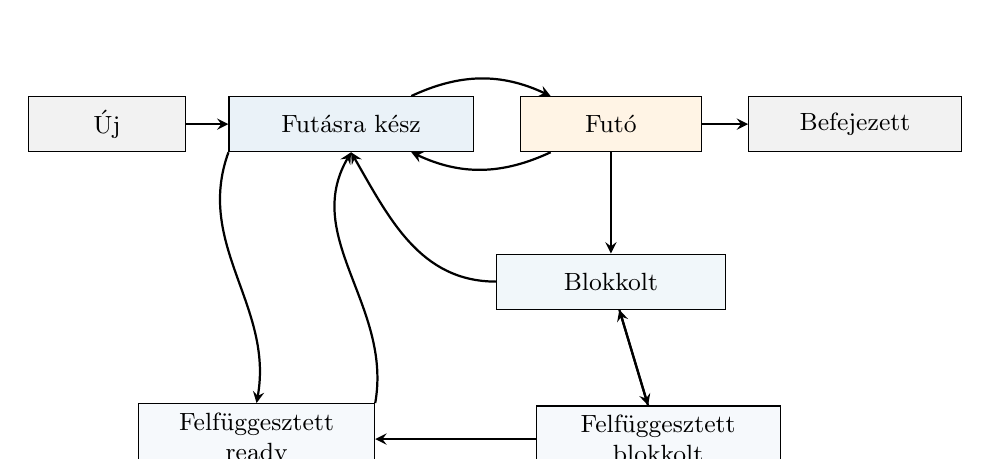
\begin{tikzpicture}[font=\small]
  \node[zvflowprocess, fill=black!5, minimum width=20mm] (new) at (0,0) {Új};
  \node[zvflowprocess, fill=lightaccent, minimum width=31mm] (ready) at (3.1,0) {Futásra kész};
  \node[zvflowprocess, fill=warnbg, minimum width=23mm] (running) at (6.4,0) {Futó};
  \node[zvflowprocess, fill=black!5, minimum width=27mm] (terminated) at (9.5,0) {Befejezett};

  \node[zvflowprocess, fill=lightaccent!65, minimum width=29mm] (blocked) at (6.4,-2.0) {Blokkolt};
  \node[zvflowprocess, fill=lightaccent!45, minimum width=30mm, align=center] (sready) at (1.9,-4.0) {Felfüggesztett\\ ready};
  \node[zvflowprocess, fill=lightaccent!45, minimum width=31mm, align=center] (sblocked) at (7.0,-4.0) {Felfüggesztett\\ blokkolt};

  \draw[arrow] (new) -- (ready);
  \draw[arrow, bend left=25] (ready) to (running);
  \draw[arrow, bend left=25] (running) to (ready);
  \draw[arrow] (running) -- (terminated);
  \draw[arrow] (running) -- (blocked);
  \draw[arrow] (blocked.west) to[out=180,in=-60] (ready.south);
  \draw[arrow] (ready.south west) to[out=-110,in=80] (sready.north);
  \draw[arrow] (sready.north east) to[out=80,in=-120] (ready.south);
  \draw[arrow] (blocked) -- (sblocked);
  \draw[arrow] (sblocked) -- (blocked);
  \draw[arrow] (sblocked) -- (sready);
\end{tikzpicture}%
}
\caption{Folyamatállapotok bővített modellje és tipikus állapotátmenetei}
\label{fig:zv16_processz_allapotmodell}
\end{figure}


A bővített modellben fontos megkülönböztetni a \textbf{blokkolt} és a \textbf{felfüggesztett} állapotot. A blokkolt folyamat azért nem fut, mert valamilyen eseményre vár. A felfüggesztett folyamatot viszont az operációs rendszer vagy a felhasználó vonta ki átmenetileg az aktív versenyből. Egy folyamat lehet egyszerre eseményre váró és felfüggesztett is.

\section{Kontextusváltás és ütemezés}

\subsection{Mikor van szükség ütemezésre?}

Ütemezésre akkor van szükség, amikor dönteni kell, hogy melyik futásra kész folyamat vagy szál kapja meg a CPU-t. Ilyen döntési helyzet például:

\begin{itemize}
  \item a futó folyamat I/O-ra vár és blokkolódik;
  \item lejár a futó folyamat időszelete;
  \item egy blokkolt folyamat eseménye befejeződik, ezért futásra kész lesz;
  \item egy folyamat befejeződik;
  \item új, magasabb prioritású feladat válik futtathatóvá.
\end{itemize}

Ha az operációs rendszer csak akkor vált, amikor a futó folyamat önként lemond a CPU-ról vagy blokkolódik, akkor \textbf{nem preemptív} ütemezésről beszélünk. Ha az operációs rendszer például órajel-megszakítás alapján kényszerítetten is elveheti a CPU-t, akkor \textbf{preemptív} ütemezésről van szó.

\subsection{Kontextusváltás menete}

Kontextusváltáskor az operációs rendszer elmenti a jelenleg futó folyamat vagy szál végrehajtási állapotát, majd visszaállítja a következő kiválasztott egység állapotát. A mentés és visszaállítás tartalmazhatja a programszámlálót, regisztereket, veremmutatót, processzállapotot, memóriakezelési információkat és ütemezési adatokat.

\begin{figure}[htbp]
\centering
\resizebox{0.95\textwidth}{!}{%
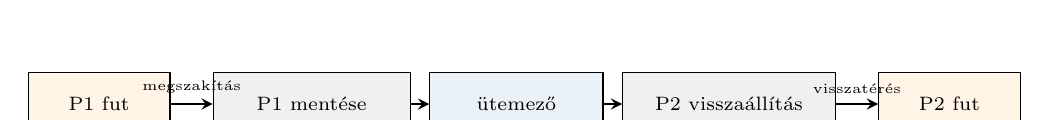
\begin{tikzpicture}[font=\scriptsize]
  \node[zvflowprocess, fill=warnbg, minimum width=18mm, minimum height=8mm] (p1run) at (0,0) {P1 fut};
  \node[zvflowprocess, fill=black!6, minimum width=25mm, minimum height=8mm] (save) at (2.7,0) {P1 mentése};
  \node[zvflowprocess, fill=lightaccent, minimum width=22mm, minimum height=8mm] (sched) at (5.3,0) {ütemező};
  \node[zvflowprocess, fill=black!6, minimum width=27mm, minimum height=8mm] (restore) at (8.0,0) {P2 visszaállítás};
  \node[zvflowprocess, fill=warnbg, minimum width=18mm, minimum height=8mm] (p2run) at (10.8,0) {P2 fut};

  \draw[arrow] (p1run) -- node[above, font=\tiny] {megszakítás} (save);
  \draw[arrow] (save) -- (sched);
  \draw[arrow] (sched) -- (restore);
  \draw[arrow] (restore) -- node[above, font=\tiny] {visszatérés} (p2run);
\end{tikzpicture}%
}
\caption{Kontextusváltás leegyszerűsített menete két folyamat között}
\label{fig:zv16_kontextusvaltas}
\end{figure}


A kontextusváltás szükséges a többfeladatos működéshez, de önmagában nem végez felhasználói szempontból hasznos munkát. Ezért az operációs rendszerek törekednek arra, hogy a váltás elég gyors legyen, és ne történjen indokolatlanul gyakran.

\section{Processz futási módok}

\subsection{Felhasználói mód és kernel mód}

A modern processzorok és operációs rendszerek rendszerint megkülönböztetnek \textbf{felhasználói módot} és \textbf{kernel módot}. Erre azért van szükség, mert a felhasználói programok nem férhetnek hozzá közvetlenül minden hardveres és rendszerbeli erőforráshoz. Ha ezt megtehetnék, egy hibás vagy rosszindulatú program könnyen tönkretehetné más folyamatok adatait vagy az egész rendszert.

\begin{itemize}
  \item \textbf{Felhasználói mód}: a folyamat korlátozott jogosultságokkal fut. Nem hajthat végre privilegizált utasításokat, és közvetlenül nem kezelheti a hardver nagy részét.
  \item \textbf{Kernel mód}: az operációs rendszer magja teljesebb jogosultságokkal fut. Itt hajthatók végre a memóriakezeléshez, I/O-hoz, megszakításkezeléshez és ütemezéshez szükséges műveletek.
\end{itemize}

A folyamat normál programkódja felhasználói módban fut. Amikor rendszerhívást végez, például fájlt olvas, memóriát kér vagy folyamatot hoz létre, vezérelt módváltás történik kernel módba. Megszakítás vagy kivétel esetén szintén a kernel veszi át a vezérlést.

\subsection{Módváltás és védelem}

A módváltás nem ugyanaz, mint a processzváltás. Rendszerhíváskor gyakran ugyanannak a folyamatnak a nevében fut kernelkód, csak magasabb jogosultsági szinten. Kontextusváltáskor viszont az operációs rendszer másik folyamat vagy szál végrehajtási állapotára vált át.

A futási módok lényege a védelem:

\begin{itemize}
  \item a felhasználói program ne módosíthassa közvetlenül a kernel memóriáját;
  \item a folyamatok címtartományai legyenek elválasztva;
  \item az I/O-eszközök kezelése ellenőrzött rendszerhívásokon keresztül történjen;
  \item a hibás program ne állíthassa le közvetlenül az egész rendszert.
\end{itemize}

\section{Szálak és fonalak}

\subsection{A szál fogalma}

A \textbf{szál} vagy \textbf{fonál} egy processzen belül létrehozott végrehajtási egység. A processz erőforrás-tulajdonosként is felfogható, a szál pedig végrehajtási útvonalnak tekinthető. Egy processz szálai ugyanazt a címtartományt használják, de mindegyiknek saját végrehajtási állapota van.

Egy szálhoz tipikusan tartozik:

\begin{itemize}
  \item saját programszámláló;
  \item saját CPU-regiszterállapot;
  \item saját verem;
  \item saját szálazonosító és ütemezési állapot.
\end{itemize}

A szálak viszont megosztják:

\begin{itemize}
  \item a processz kódterületét;
  \item a globális adatokat és a heapet;
  \item a nyitott fájlokat és egyéb processzszintű erőforrásokat;
  \item a processz jogosultsági és címtérbeli kereteit.
\end{itemize}

\begin{figure}[htbp]
\centering
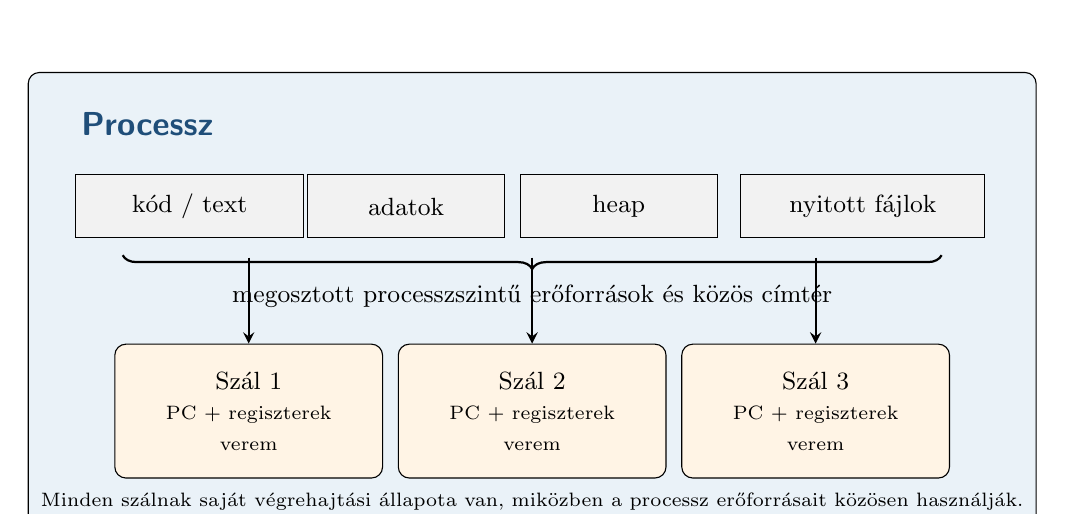
\begin{tikzpicture}[font=\small]
  \node[draw, rounded corners, fill=lightaccent, minimum width=12.8cm, minimum height=5.8cm] (proc) at (0,0) {};
  \node[anchor=west, font=\bfseries\sffamily\large, color=accent] at (-5.85,2.25) {Processz};

  \node[zvflowprocess, fill=black!5, minimum width=29mm, minimum height=8mm] (code) at (-4.35,1.2) {kód / text};
  \node[zvflowprocess, fill=black!5, minimum width=25mm, minimum height=8mm] (data) at (-1.6,1.2) {adatok};
  \node[zvflowprocess, fill=black!5, minimum width=25mm, minimum height=8mm] (heap) at (1.1,1.2) {heap};
  \node[zvflowprocess, fill=black!5, minimum width=31mm, minimum height=8mm] (files) at (4.2,1.2) {nyitott fájlok};

  \draw[decorate, decoration={brace, mirror, amplitude=5pt}, thick]
    (-5.2,0.58) -- (5.2,0.58)
    node[midway, below=7pt, align=center] {megosztott processzszintű erőforrások és közös címtér};

  \node[draw, rounded corners, fill=warnbg, minimum width=34mm, minimum height=17mm, align=center] (t1) at (-3.6,-1.4) {Szál 1\\{\scriptsize PC + regiszterek}\\{\scriptsize verem}};
  \node[draw, rounded corners, fill=warnbg, minimum width=34mm, minimum height=17mm, align=center] (t2) at (0,-1.4) {Szál 2\\{\scriptsize PC + regiszterek}\\{\scriptsize verem}};
  \node[draw, rounded corners, fill=warnbg, minimum width=34mm, minimum height=17mm, align=center] (t3) at (3.6,-1.4) {Szál 3\\{\scriptsize PC + regiszterek}\\{\scriptsize verem}};

  \draw[arrow] (-3.6,0.55) -- (t1.north);
  \draw[arrow] (0,0.55) -- (t2.north);
  \draw[arrow] (3.6,0.55) -- (t3.north);

  \node[font=\scriptsize, align=center] at (0,-2.55) {Minden szálnak saját végrehajtási állapota van, miközben a processz erőforrásait közösen használják.};
\end{tikzpicture}
\caption{Processz és szál kapcsolata: közös erőforrások, saját végrehajtási állapot}
\label{fig:zv16_processz_es_szal_eroforrasok}
\end{figure}


\subsection{Miért előnyösek a szálak?}

A szálak használatának több gyakorlati előnye van:

\begin{itemize}
  \item \textbf{gyorsabb reakció}: ha egy szál I/O-ra vár, a processz más szálai még dolgozhatnak;
  \item \textbf{olcsóbb vezérlés}: szálat létrehozni és szálak között váltani általában olcsóbb, mint teljes processzek között;
  \item \textbf{erőforrás-megosztás}: a szálak közös memóriát és fájlokat használhatnak;
  \item \textbf{párhuzamosság}: többmagos rendszeren több szál ténylegesen párhuzamosan futhat;
  \item \textbf{természetes feladatfelbontás}: például egy médialejátszóban külön szál kezelheti a hangot, a videót, a hálózatot és a felhasználói felületet.
\end{itemize}

A közös címtér miatt ugyanakkor a szálak veszélyesebbek is lehetnek: ha több szál ugyanazt az adatot módosítja, szinkronizáció nélkül versenyhelyzet, inkonzisztens állapot vagy holtpont alakulhat ki.

\begin{center}
\begin{tabularx}{\textwidth}{L{32mm}X X}
\toprule
\textbf{Szempont} & \textbf{Processz} & \textbf{Szál / fonál} \\
\midrule
Alapjelentés & Program végrehajtás alatti példánya. & Végrehajtási út egy processzen belül. \\
Címtér & Általában saját, védett címtérrel rendelkezik. & Megosztja a processz címtérét a többi szállal. \\
Saját adatok & PCB, címtér, nyitott erőforrások, legalább egy végrehajtási szál. & Saját programszámláló, regiszterállapot és verem. \\
Erőforrás-megosztás & Processzek között drágább és szabályozottabb, például IPC kellhet. & Azonos processzen belüli szálak könnyen megosztják a kódot, adatokat, heapet és fájlokat. \\
Létrehozás és váltás költsége & Általában drágább, mert több erőforrás és több védelmi információ kapcsolódik hozzá. & Általában olcsóbb, ezért nevezik könnyűsúlyú folyamatnak is. \\
Hibatűrés & Egy processz hibája gyakran elszigetelhető más processzektől. & Egy szál hibája az egész processzt érintheti, mert közös címtéren osztoznak. \\
\bottomrule
\end{tabularx}

\end{center}

\subsection{Felhasználói és kernel szintű szálak}

A szálak megvalósítása alapján két alapvető eset különíthető el. \textbf{Felhasználói szintű szálaknál} a szálkezelést egy felhasználói könyvtár végzi, ezért az operációs rendszer gyakran csak a teljes processzt látja. \textbf{Kernel szintű szálaknál} az operációs rendszer ismeri és külön ütemezi a szálakat.

\begin{center}
\begin{tabularx}{\textwidth}{L{34mm}X X}
\toprule
\textbf{Típus} & \textbf{Jellemző} & \textbf{Következmény} \\
\midrule
Felhasználói szintű szál & A szálakat felhasználói könyvtár kezeli, az operációs rendszer csak a processzt látja. & A szálváltás gyors lehet, de ha egy szál blokkoló rendszerhívást végez, az egész processz blokkolódhat. \\
Kernel szintű szál & A szálakat az operációs rendszer kernelje ismeri és ütemezi. & Egy szál blokkolása nem feltétlenül állítja meg a processz többi szálát; a váltás viszont drágább lehet. \\
Egy--több modell & Több felhasználói szál tartozik egy kernel végrehajtási egységhez. & Egyszerű, de valódi többmagos párhuzamosságot korlátozottan ad. \\
Egy--egy modell & Minden felhasználói szálhoz külön kernel szál tartozik. & Jó párhuzamosságot ad, de sok kernel szál erőforrásigényes lehet. \\
Több--több modell & Több felhasználói szál több kernel szálra képeződik le. & Rugalmasabb, de bonyolultabb megvalósítani. \\
\bottomrule
\end{tabularx}

\end{center}

Ha a szálak csak felhasználói szinten léteznek, akkor egy blokkoló rendszerhívás az egész processzt megállíthatja, mert az operációs rendszer nem látja a processzen belüli többi futtatható szálat. Kernel szintű szálaknál az operációs rendszer egy másik szálat is futtathat ugyanabból a processzből, amíg az egyik szál várakozik.

\section{Taszk- és fonálállapotok}

\subsection{Taszkállapotok}

A taszk állapotmodellje általában hasonló a processz állapotmodelljéhez, mert a taszk is végrehajtandó vagy ütemezendő egységet jelent. A leggyakoribb állapotok:

\begin{itemize}
  \item \textbf{created / new}: a taszk létrejött;
  \item \textbf{ready}: futtatható, CPU-ra vár;
  \item \textbf{running}: éppen végrehajtás alatt van;
  \item \textbf{waiting / blocked}: eseményre, erőforrásra vagy I/O-ra vár;
  \item \textbf{suspended}: átmenetileg kivonták az ütemezésből;
  \item \textbf{terminated}: befejeződött.
\end{itemize}

Az átmenetek oka lehet indítás, ütemezői kiválasztás, időszelet lejárta, várakozás kezdete, esemény bekövetkezése, felfüggesztés, folytatás vagy befejezés. Valós idejű operációs rendszerekben a taszk fogalom különösen gyakori, mert ott a feladatok határidővel, prioritással és eseményekre adott reakcióval kapcsolódnak össze.

\subsection{Fonálállapotok}

A fonál vagy szál állapotai a processzállapotokhoz hasonlítanak, de az állapot a processzen belüli végrehajtási útra vonatkozik. Egy többszálú processzben elképzelhető, hogy az egyik szál blokkolt, miközben egy másik szál ugyanazon processzen belül futásra kész vagy futó állapotban van.

Tipikus fonálállapotok:

\begin{itemize}
  \item \textbf{új}: a szál objektuma vagy leírója létrejött, de még nem indult el;
  \item \textbf{futásra kész}: a szál végrehajtható, CPU-ra vár;
  \item \textbf{futó}: a szál CPU-n van;
  \item \textbf{blokkolt vagy várakozó}: zárolásra, I/O-ra, időzítőre vagy másik szál jelzésére vár;
  \item \textbf{befejezett}: a szál futása véget ért.
\end{itemize}

A fontos átmenetek:

\begin{itemize}
  \item indítás után a szál futásra kész lesz;
  \item az ütemező futásra kész szálat választ, így futó állapotba kerül;
  \item időszelet lejártakor vagy magasabb prioritású szál megjelenésekor visszakerülhet futásra kész állapotba;
  \item I/O, zárolás vagy várakozás miatt blokkolódhat;
  \item a várt esemény bekövetkezése után ismét futásra kész lesz;
  \item a szálfüggvény végén befejezett állapotba kerül.
\end{itemize}

\begin{warningbox}
Vizsgán érdemes külön kiemelni: ha a szálak kernel szintűek, akkor egy szál blokkolódása nem feltétlenül blokkolja az egész processzt. Ha viszont a szálakat csak felhasználói szintű könyvtár kezeli, akkor egy blokkoló rendszerhívás az egész processzt megakaszthatja.
\end{warningbox}

\section{Gyakori vizsgahibák és összefoglalás}

\subsection{Gyakori félreértések}

\begin{itemize}
  \item \textbf{A program és a processz nem ugyanaz.} A program statikus, a processz futó példány.
  \item \textbf{A blokkolt folyamat nem azért nem fut, mert nincs kiválasztva.} A blokkolt folyamat valamilyen eseményre vár, ezért akkor sem lenne futtatható, ha lenne szabad CPU.
  \item \textbf{A ready állapot nem jelent futást.} A folyamat készen áll a futásra, de még vár a CPU-ra.
  \item \textbf{A módváltás nem azonos a kontextusváltással.} Kernel módba át lehet lépni ugyanannak a folyamatnak a nevében is.
  \item \textbf{A szál nem teljesen önálló processz.} Saját végrehajtási állapota van, de sok erőforrást megoszt a processz többi szálával.
  \item \textbf{A szálak közötti közös memória előny és veszély is.} Gyors kommunikációt ad, de szinkronizáció nélkül versenyhelyzetet okozhat.
\end{itemize}

\subsection{Rövid vizsgaválasz-minta}

\begin{summarybox}
A processz egy program végrehajtás alatti példánya, amelyet az operációs rendszer hoz létre, ütemez, nyilvántart és szüntet meg. A processzhez saját címtér, erőforrások és PCB tartozik. A PCB tartalmazza többek között a processz azonosítóját, állapotát, programszámlálóját, regisztereit, ütemezési, memória- és I/O-adatait. A folyamat kontextusa teszi lehetővé a kontextusváltást: az operációs rendszer elmenti a futó folyamat állapotát, majd egy másik folyamat vagy szál állapotát állítja vissza. A fő folyamatállapotok: új, futásra kész, futó, blokkolt, felfüggesztett és befejezett. A szál a processzen belüli végrehajtási egység, amely saját programszámlálóval, regiszterekkel és veremmel rendelkezik, de megosztja a processz kódját, adatait, heapjét és nyitott erőforrásait. A futási módok közül felhasználói módban korlátozott jogosultságú programkód fut, kernel módban pedig az operációs rendszer privilegizált műveletei hajtódnak végre.
\end{summarybox}

\end{document}
